\documentclass[aspectratio=169]{beamer}
\setbeamertemplate{navigation symbols}{}
\usepackage{color,amsmath,comment, subfigure}
\usepackage{booktabs}
\def\vf{\vfill}
\usepackage{url}

%\setbeameroption{show notes}

%%%%%%%%%%%%%%%%%%%%%%%%%%
\title[]{Lecture 6: Foci}
\author[]{Matthew Salganik}
\institute[]{Sociology 204: Social Networks, Spring 2021\\Princeton University}
\date[]{
1/3: Lois Weisberg and social structure

\vfill

\begin{flushleft}
\vspace{0.7in}

\includegraphics[width=0.05\textwidth]{figures/cc.png}
\end{flushleft}
}

\begin{document}
%%%%%%%%%%%%%%%%%%%%%%%%%%%
\frame{\titlepage}
%%%%%%%%%%%%%%%%%%%%%%%%%%%
\begin{comment}
\begin{frame}

SWBAT:
\begin{enumerate}
\item realize the power of edges that don't exist
\item compare psychological vs sociological explanations for network structure
\item apply the idea of foci to understand their personal networks 
\item see how sociological principles can shape the design of technical systems
\end{enumerate}

\end{frame}
\end{comment}
%%%%%%%%%%%%%%%%%%%%%%%%
\begin{frame}
\frametitle{Review}

\begin{itemize}
\item growth + preferential attachment $\rightarrow$ power law degree distribution
\pause
\item some (but not all) real networks have a power law degree distribution 
\pause
\item diseases spread more easily on networks with power law degree distribution than on other types of networks
\pause
\item networks with power law degree distribution are robust to random failure but fragile to targeted attack
\pause
\item ``hubs'' seem important
\end{itemize}

\end{frame}
%%%%%%%%%%%%%%%%%%%%%%%
\begin{frame}

\begin{figure}
  \centering
  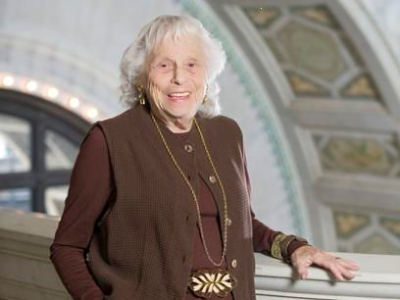
\includegraphics[width=0.7\textwidth]{figures/lois_weisberg}
\end{figure}

Her story connects 2 ideas: power law degree distributions and foci
\vfill

\tiny{Source: \url{www.wbez.org}}

\note{
Lois Weisberg is a ``connector'' (something Gladwell talks about more in tipping point).  For our purposes Lois also connects two ideas: power law degree distributions and foci.  ``It is not nearly that she knows lots of people.  It is that she belongs to lots of different worlds.''  Lois belonged to eight worlds: the actors, the writers, the doctors, the lawyers, the park lovers, the politicians, the railroad bugs, and the flea-market aficionados.  Thus it is not just her ties, but the lack of ties between her friends.  In other words we have talked about ties, now we are going to talk about lack of ties.
}

\end{frame}
%%%%%%%%%%%%%%%%%%%%%%%%%%%%
\begin{frame}

``It is not nearly that she knows lots of people.  It is that she belongs to lots of different worlds.'' 
\pause
\begin{itemize}
\item the actors
\pause
\item the writers
\pause
\item the doctors
\pause
\item the lawyers
\pause
\item the park lovers
\pause
\item the politicians
\pause
\item the railroad bugs
\pause
\item the flea-market aficionados
\end{itemize}

\pause
\vfill
A key point is that these people don't know each other. That enables Lois to be a ``broker.''
\note{
Not just her connections but the lack of connections between people she knows
}

\end{frame}
%%%%%%%%%%%%%%%%%%%%%%%%%%%%
\begin{frame}

\begin{figure}
  \centering
  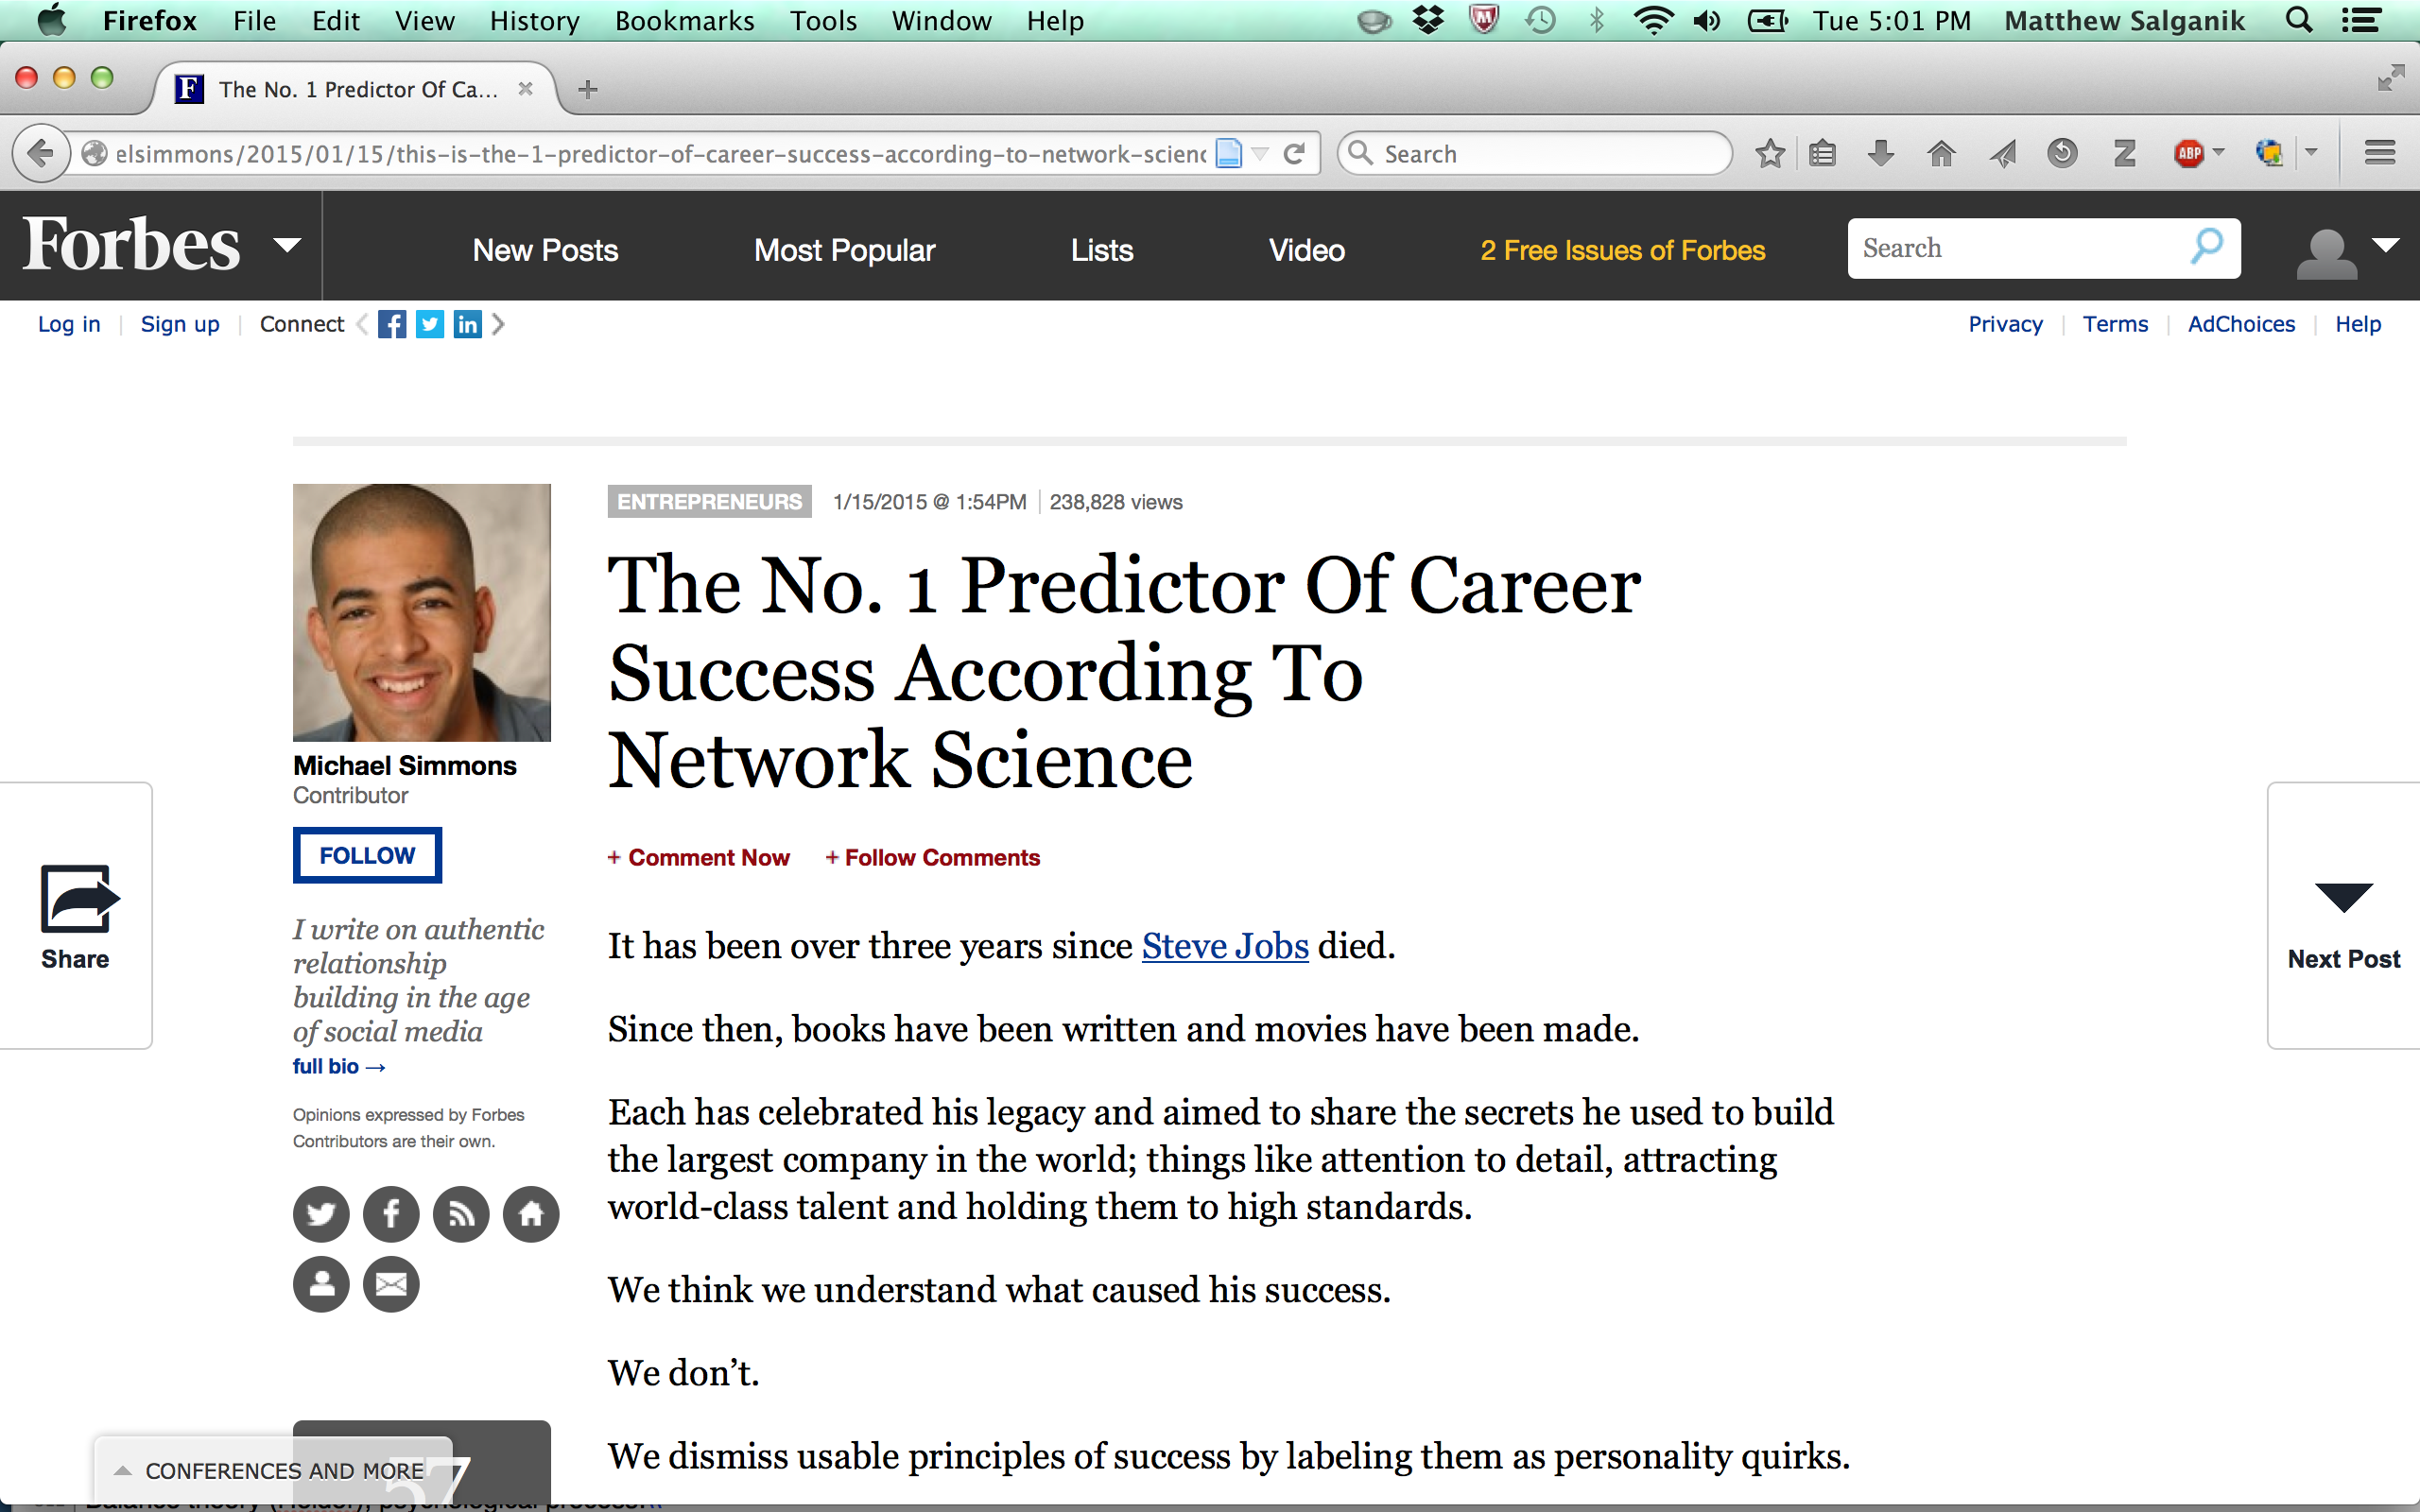
\includegraphics[width=0.9\textwidth]{figures/simmons_predictor_2015}
\end{figure}

\tiny{Source: \url{http://www.forbes.com/sites/michaelsimmons/2015/01/15/this-is-the-1-predictor-of-career-success-according-to-network-science/}}

\note{open networks are good in firms}

\end{frame}
%%%%%%%%%%%%%%%%%%%%%%%%%%%%
\begin{frame}

\begin{figure}
  \centering
  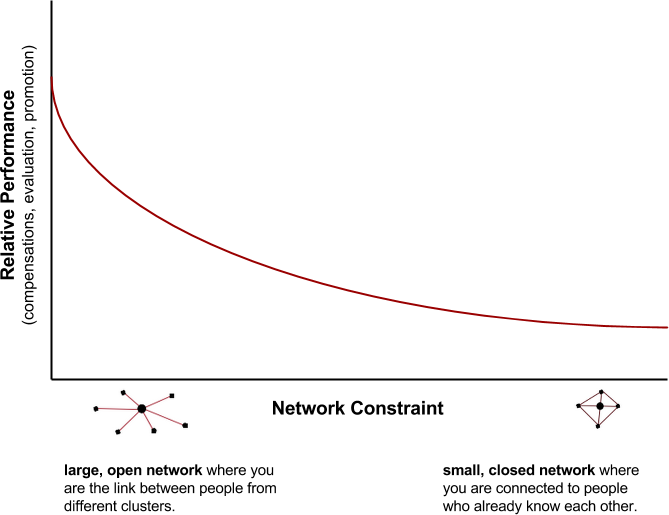
\includegraphics[width=0.8\textwidth]{figures/Burt_Success_Final.png}
\end{figure}

\tiny{Source: \url{http://www.forbes.com/sites/michaelsimmons/2015/01/15/this-is-the-1-predictor-of-career-success-according-to-network-science/}}

\note{open networks are good in firms}

\end{frame}
%%%%%%%%%%%%%%%%%%%%%%%%%%%%
\begin{frame}

\begin{figure}
  \centering
  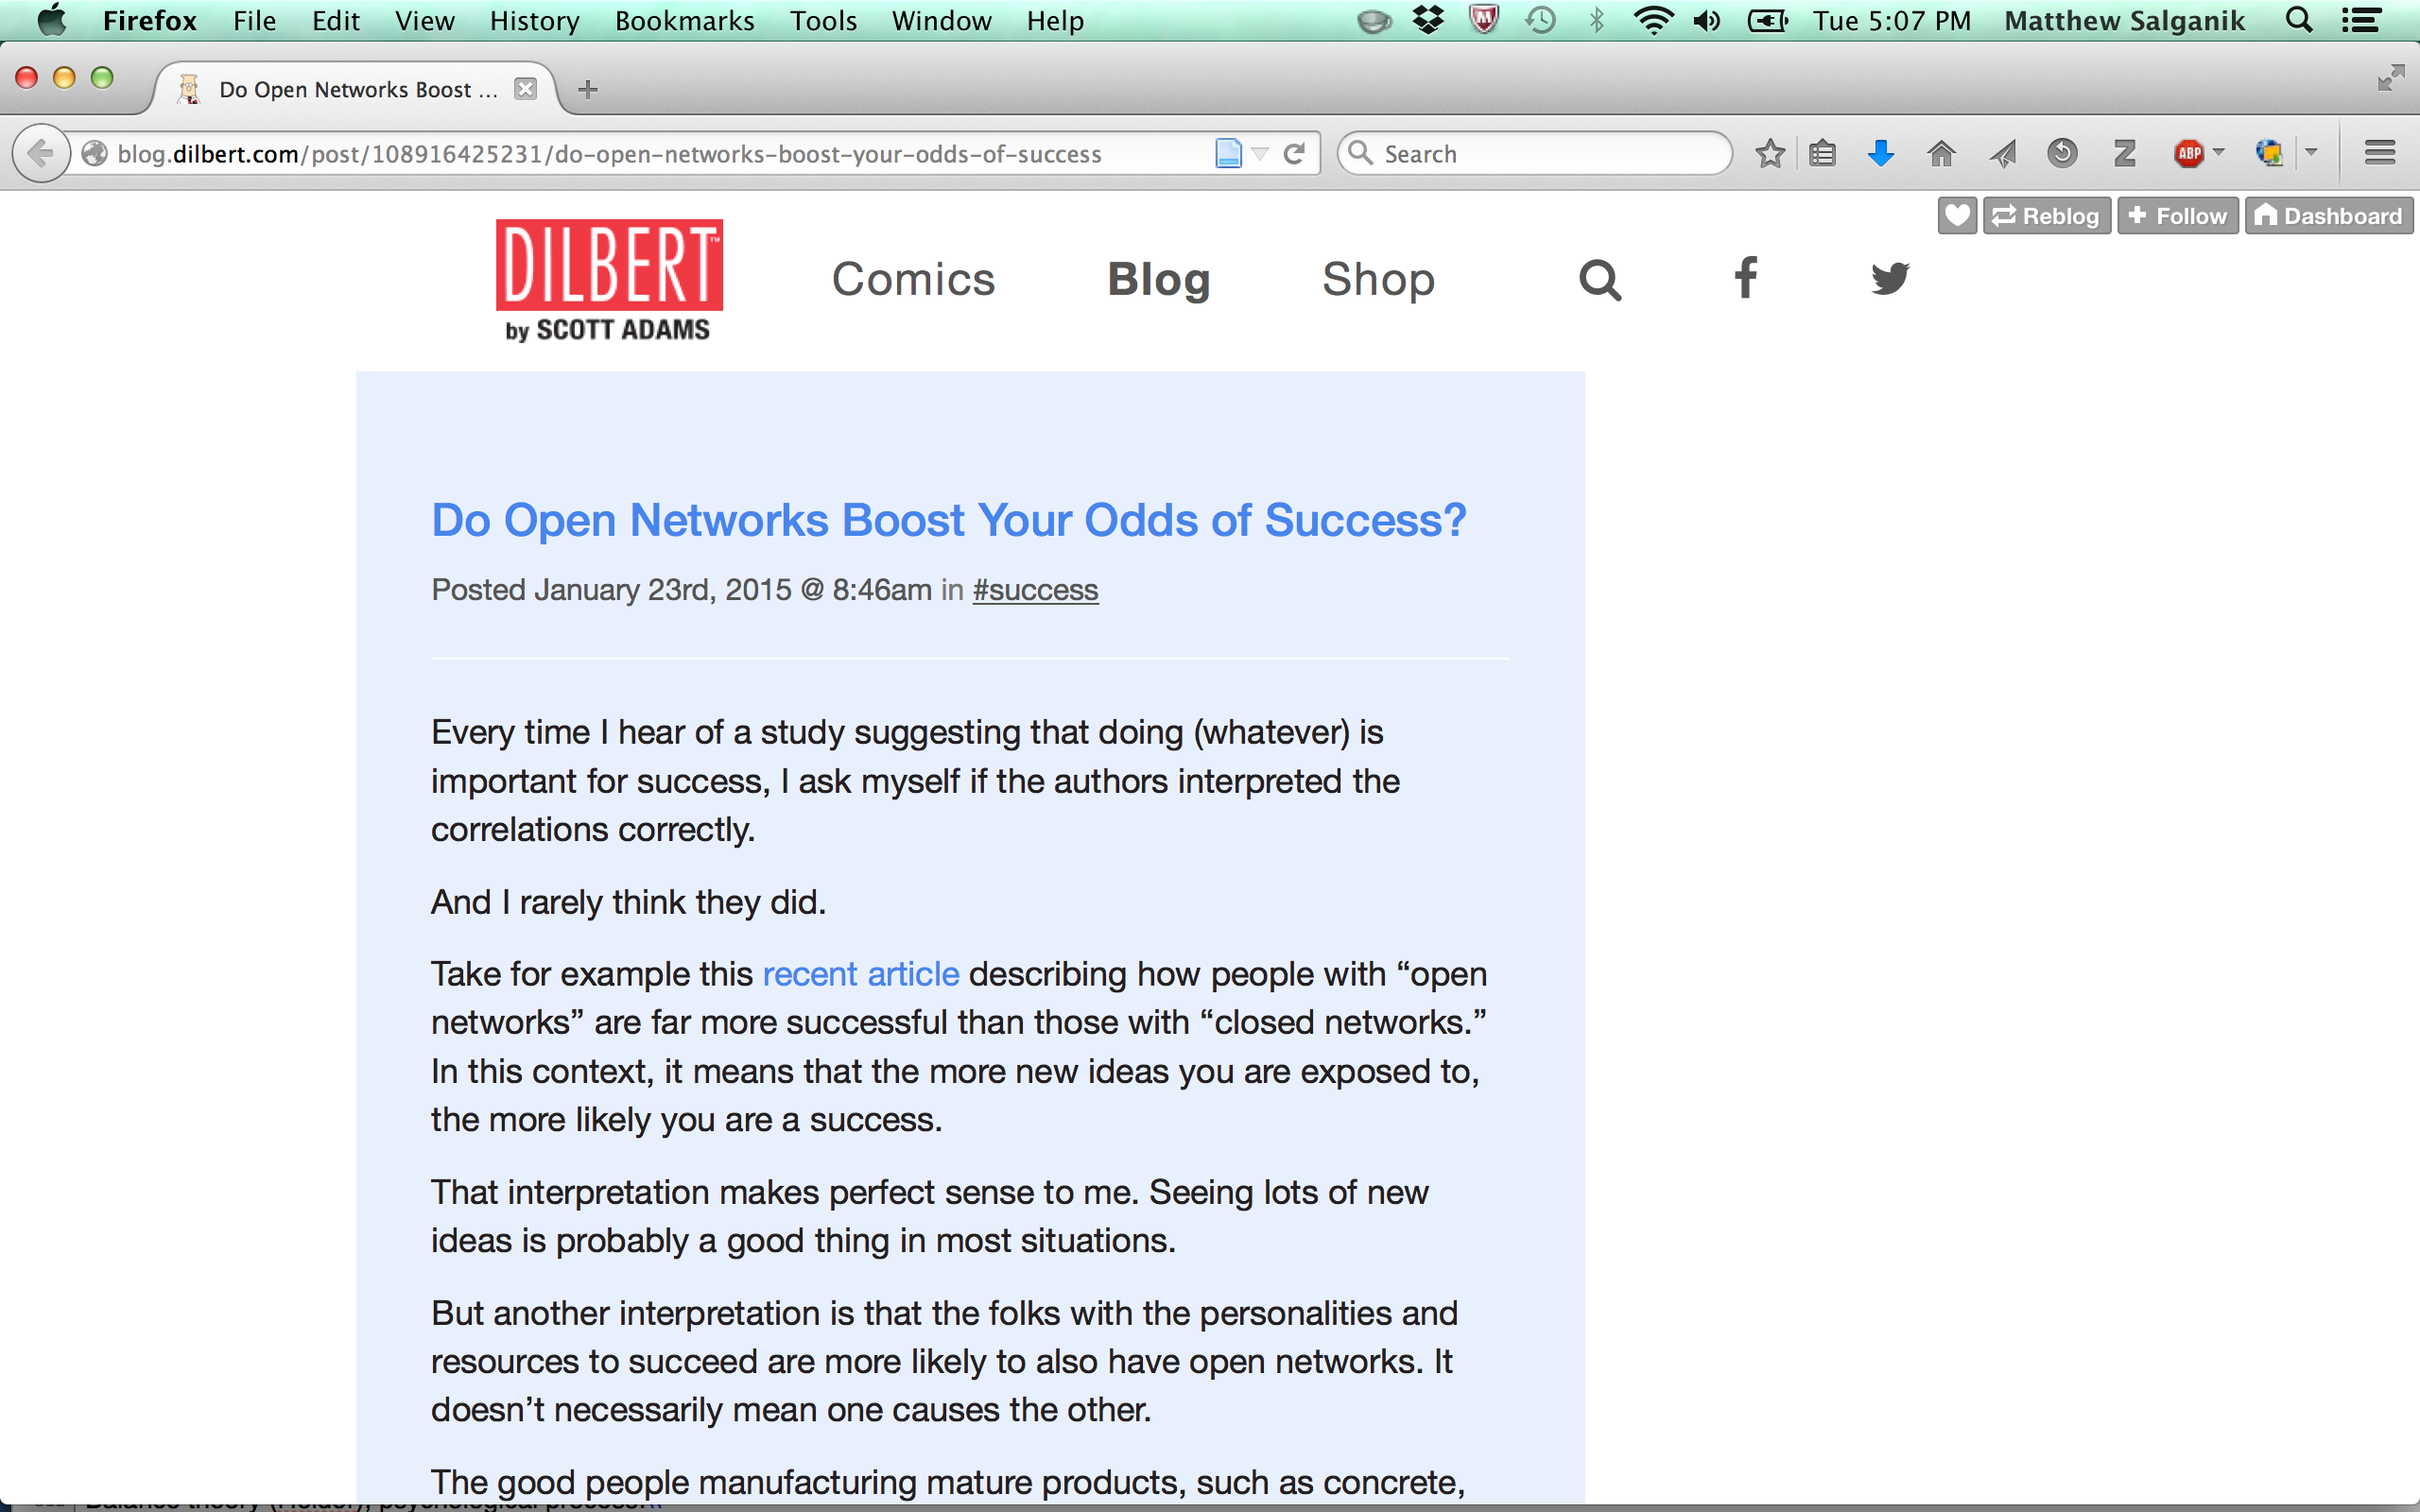
\includegraphics[width=0.9\textwidth]{figures/adams_do_2015}
\end{figure}

\tiny{Source: \url{http://blog.dilbert.com/post/108916425231/do-open-networks-boost-your-odds-of-success}}

\note{correlation is not causation}

\end{frame}
%%%%%%%%%%%%%%%%%%%%%%%%%%%%
\begin{frame}

\begin{figure}
  \centering
  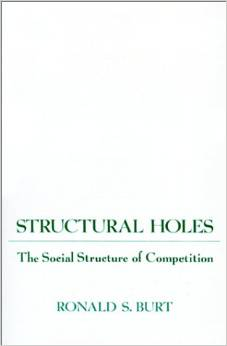
\includegraphics[height=0.8\textheight]{figures/burt_structural_1995}
\end{figure}

\note{For the real details see Burt}

\end{frame}
%%%%%%%%%%%%%%%%%%%%%%%%%%%
\begin{frame}

How does Lois Weisberg's story---and the readings more generally---change how we should think about networks?

\pause 

Combines:
\begin{itemize}
\item network structure
\item social structure 
\end{itemize}

\note{
What is social structure?  For our purposes groups.
In the next video we will learn about how Watts and Feld think about social structure
}

\end{frame}

\end{document}
